\documentclass[11pt]{article}
\usepackage[letterpaper,margin=0.82in]{geometry}
\usepackage{amsmath,amssymb,amsthm,mathtools}
\usepackage{graphicx}
\usepackage{microtype}
\usepackage{xcolor}
\usepackage[hidelinks]{hyperref}

\definecolor{softgray}{RGB}{245,247,250}
\newtheorem{theorem}{Theorem}
\newtheorem{lemma}[theorem]{Lemma}
\newcommand{\C}{\mathbb C}
\newcommand{\B}{\mathbb B}
\newcommand{\K}{\mathcal K}
\newcommand{\ran}{\operatorname{ran}}

\title{\vspace{-2.5em}\textbf{Principal polynomial submodule projections need not almost commute}\\
\large A counterexample to the question in arXiv:1204.0620}
\author{Candidate solution packet --- run \texttt{fa\_banach\_001}, lane 2}
\date{27 August 2026}

\begin{document}
\maketitle

\noindent
\colorbox{softgray}{\parbox{0.95\linewidth}{
\textbf{Status.} Candidate counterexample, likely valid; human review is
recommended. In every dimension $n\ge3$, the projections onto the principal
submodules generated by $z_1$ and $z_1+z_2$ fail to commute modulo compact
operators in each of the Hardy, Bergman, and Drury--Arveson modules on the
unit ball.}}

\section{Source question}

Douglas and Wang ask whether the projections onto two principal polynomial
submodules might always almost commute \cite{DW}. Their paragraph begins at
the bottom of printed page 7 and continues on printed page 8:

\begin{center}

\includegraphics[width=0.96\linewidth]{figures/open_problem_crop.png}

\vspace{0.35em}
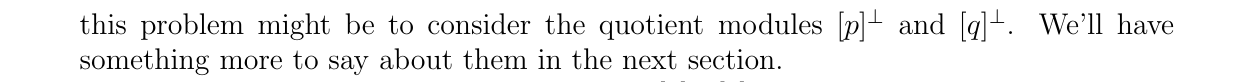
\includegraphics[width=0.96\linewidth]{figures/open_problem_continuation.png}
\end{center}

The exact suggestion is:
\begin{quote}
For polynomials $p,q\in\C[z_1,\ldots,z_n]$, if $P_{[p]}$ and $P_{[q]}$
are the orthogonal projections onto the closures of the corresponding
principal ideals in the Hardy, Bergman, or Drury--Arveson module on the unit
ball, is $[P_{[p]},P_{[q]}]$ always compact?
\end{quote}
Here ``almost commute'' means membership of the commutator in the compact
operator ideal $\K$.

\section{Setup}

Let $\mathcal H$ be one of the following Hilbert modules on $\B^n$:
the Hardy module $H^2(\partial\B^n)$, the Bergman module
$A^2(\B^n)$, or the Drury--Arveson module $H_n^2$.  Each is an orthogonal
sum of its finite-dimensional homogeneous pieces,
\[
                    \mathcal H=\bigoplus_{m\ge0}\mathcal H_m.
\]
The monomials form an orthogonal basis, and for $|\alpha|=m$ their squared
norms have the form
\begin{equation}\label{eq:norms}
                       \|z^\alpha\|^2=c_m\,\alpha!,
\end{equation}
where $c_m>0$ depends on the module and on $m$, but not on the arrangement of
the coordinates of $\alpha$.  In particular, exchanging $z_1$ and $z_2$
preserves monomial norms.

For a polynomial $r$, write $[r]$ for the closure of $r\C[z_1,\ldots,z_n]$
in $\mathcal H$, and $P_{[r]}$ for its orthogonal projection.

\section{Proof intuition}

The source's positive criterion applies when the two boundary zero varieties
are disjoint.  Two transverse hyperplanes in dimension at least three meet
along a nontrivial boundary set, and that common direction lets the same
two-dimensional angle recur in every homogeneous degree.  Concretely, the
factor $z_3^{m-1}$ carries the angle between $z_1$ and $z_1+z_2$ unchanged
through all degrees.  The quotient projections therefore contain infinitely
many identical $2\times2$ blocks, each with commutator norm $1/2$.

\section{Counterexample}

\begin{theorem}\label{thm:counterexample}
Let $n\ge3$, and let $\mathcal H$ be the Hardy, Bergman, or Drury--Arveson
module on $\B^n$. Set
\[
                    p=z_1,\qquad q=z_1+z_2.
\]
If $P=P_{[p]}$ and $Q=P_{[q]}$, then $[P,Q]\notin\K(\mathcal H)$. More
precisely, $[P,Q]$ has a reducing two-dimensional block of norm $1/2$ in
every positive homogeneous degree.
\end{theorem}

\begin{proof}
Put $E=I-P$ and $F=I-Q$, the orthogonal projections onto $[p]^\perp$ and
$[q]^\perp$. Since
\[
              [I-E,I-F]=EF-FE=[E,F],
\]
it is enough to prove that $[E,F]$ is not compact.

For every $m\ge1$, define
\[
 u_m=z_1z_3^{m-1},\qquad v_m=z_2z_3^{m-1},\qquad
 V_m=\operatorname{span}\{u_m,v_m\}\subset\mathcal H_m.
\]
By \eqref{eq:norms}, $u_m$ and $v_m$ are orthogonal and have equal norm.
We use the normalized ordered basis $(e_m,f_m)$ obtained from $(u_m,v_m)$.

The degree-$m$ part of $[z_1]$ is spanned by the degree-$m$ monomials which
are divisible by $z_1$. Thus $u_m\in[z_1]$, while $v_m$ is orthogonal to the
whole degree-$m$ part of $[z_1]$. Consequently $V_m$ reduces $E$ and
\begin{equation}\label{eq:E}
                  E|_{V_m}=\begin{pmatrix}0&0\\0&1\end{pmatrix}.
\end{equation}

Next,
\[
             u_m+v_m=(z_1+z_2)z_3^{m-1}\in[q].
\]
On the other hand, $u_m-v_m$ is orthogonal to $[q]\cap\mathcal H_m$.
Indeed, if $r$ is a degree-$(m-1)$ monomial other than $z_3^{m-1}$, then
both monomials in $(z_1+z_2)r$ are orthogonal to $u_m$ and $v_m$; for
$r=z_3^{m-1}$, equal norms give
\[
       \langle u_m-v_m,u_m+v_m\rangle=\|u_m\|^2-\|v_m\|^2=0.
\]
By linearity this holds for every homogeneous polynomial $r$ of degree
$m-1$. Hence $V_m$ also reduces $F$, and $F|_{V_m}$ is the projection onto
the normalized difference $(e_m-f_m)/\sqrt2$:
\begin{equation}\label{eq:F}
                  F|_{V_m}=\frac12\begin{pmatrix}1&-1\\-1&1\end{pmatrix}.
\end{equation}
Combining \eqref{eq:E} and \eqref{eq:F},
\begin{equation}\label{eq:commutator}
 [P,Q]|_{V_m}=[E,F]|_{V_m}
 =\begin{pmatrix}0&\tfrac12\\-\tfrac12&0\end{pmatrix},
 \qquad \|[P,Q]|_{V_m}\|=\frac12.
\end{equation}

The vectors $e_m$ are orthonormal as $m$ varies because they lie in distinct
homogeneous degrees, while \eqref{eq:commutator} gives
$\|[P,Q]e_m\|=1/2$ for every $m$. An orthonormal sequence is weakly null,
and a compact operator sends weakly null bounded sequences to norm-null
sequences. Therefore $[P,Q]$ is not compact.
\end{proof}

\section{Verification, scope, and novelty}

\paragraph{Verification.}
The argument uses only three exact facts: orthogonality of distinct monomials,
equality of the two monomial norms under coordinate exchange, and the graded
description of a principal submodule generated by a linear homogeneous
polynomial. These hold in all three named modules. The two matrices in
\eqref{eq:E}--\eqref{eq:F} multiply to the skew matrix in
\eqref{eq:commutator}; no numerical or asymptotic estimate is involved.

\paragraph{Scope.}
The counterexample disproves the unrestricted ``always'' suggestion for every
$n\ge3$. It does not decide dimensions $n=1,2$. The zero varieties of $z_1$
and $z_1+z_2$ meet on $\partial\B^n$ when $n\ge3$, so the example does not
contradict the source's positive disjoint-boundary-variety result.

\paragraph{Bounded novelty search.}
On 27 August 2026, searches used arXiv:1204.0620, the exact paper title and
authors, the phrases ``projections onto $[p]$ and $[q]$ almost commute'' and
``principal polynomial submodules projection commutator compact'', and the
specific pair $z_1,z_1+z_2$. The searches found the source and later work on
essential normality of individual polynomial-generated submodules, but no
paper stating this counterexample or resolving this pairwise-projection
question. This supports, but does not prove, novelty.

\paragraph{Human-review recommendation.}
Verify the restrictions of $E$ and $F$ to $V_m$, especially the orthogonality
of $u_m-v_m$ to $(z_1+z_2)\mathcal H_{m-1}$. Once that two-line calculation is
confirmed, noncompactness is immediate.

\begin{thebibliography}{9}
\bibitem{DW}
R. G. Douglas and K. Wang,
\emph{Some Remarks On Essentially Normal Submodules},
arXiv:1204.0620 (2012); published in \emph{Concrete Operators, Spectral
Theory, Operators in Harmonic Analysis and Approximation}, Operator Theory:
Advances and Applications 236, Birkh\"auser, 2014, pp. 159--170.
\end{thebibliography}

\end{document}

